%%%%%%%%%%%%%%%%%%%%%%%%%%%%%%%%%%%%%%%%%
% Beamer Presentation
% LaTeX Template
% Version 1.0 (10/11/12)
%
% This template has been downloaded from:
% http://www.LaTeXTemplates.com
%
% License:
% CC BY-NC-SA 3.0 (http://creativecommons.org/licenses/by-nc-sa/3.0/)
%
%%%%%%%%%%%%%%%%%%%%%%%%%%%%%%%%%%%%%%%%%

%----------------------------------------------------------------------------------------
%	PACKAGES AND THEMES
%----------------------------------------------------------------------------------------

\documentclass[aspectratio=169]{beamer}
\usetheme[progressbar=frametitle]{metropolis}
\usepackage{appendixnumberbeamer}


\usepackage{caption}
\usepackage{subcaption}

\usepackage[backend=biber, citestyle=authoryear, bibencoding=utf8]{biblatex}
\addbibresource{../bibs/vlab-report.bib}
\addbibresource{../bibs/unicef-ie.bib}

\mode<presentation> {

% The Beamer class comes with a number of default slide themes
% which change the colors and layouts of slides. Below this is a list
% of all the themes, uncomment each in turn to see what they look like.

%\usetheme{default}
%\usetheme{AnnArbor}
%\usetheme{Antibes}
%\usetheme{Bergen}
%\usetheme{Berkeley}
%\usetheme{Berlin}
% \usetheme{Boadilla} %
%\usetheme{CambridgeUS} %
%\usetheme{Copenhagen}
%\usetheme{Darmstadt}
%\usetheme{Dresden}
%\usetheme{Frankfurt}
%\usetheme{Goettingen}
%\usetheme{Hannover}
%\usetheme{Ilmenau}
%\usetheme{JuanLesPins}
%\usetheme{Luebeck}
%\usetheme{Madrid} %
%\usetheme{Malmoe}
%\usetheme{Marburg}
%\usetheme{Montpellier}
%\usetheme{PaloAlto}
%\usetheme{Pittsburgh}
%\usetheme{Rochester}
%\usetheme{Singapore} %
%\usetheme{Szeged}
%\usetheme{Warsaw}

% As well as themes, the Beamer class has a number of color themes
% for any slide theme. Uncomment each of these in turn to see how it
% changes the colors of your current slide theme.

%\usecolortheme{albatross}
%\usecolortheme{beaver} %
%\usecolortheme{beetle}
%\usecolortheme{crane}
%\usecolortheme{dolphin}
%\usecolortheme{dove}
%\usecolortheme{fly}
%\usecolortheme{lily}
%\usecolortheme{orchid}
%\usecolortheme{rose}
%\usecolortheme{seagull}
%\usecolortheme{seahorse}
%\usecolortheme{whale}
%\usecolortheme{wolverine}

%\setbeamertemplate{footline} % To remove the footer line in all slides uncomment this line
%\setbeamertemplate{footline}[page number] % To replace the footer line in all slides with a simple slide count uncomment this line

\setbeamertemplate{navigation symbols}{} % To remove the navigation symbols from the bottom of all slides uncomment this line
}

\usepackage{graphicx} % Allows including images
\usepackage{booktabs} % Allows the use of \toprule, \midrule and \bottomrule in tables

\usepackage{accents}
\newcommand{\ubar}[1]{\underaccent{\bar}{#1}}
\usepackage{stmaryrd}


\usepackage{pgfplots}
\pgfplotsset{width=7cm,compat=1.9}

\usepackage{tabularx}
\newcolumntype{Y}{>{\centering\arraybackslash}X}\newcolumntype{Y}{>{\centering\arraybackslash}X}
	\newcommand\fnote[1]{\captionsetup{font=footnotesize}\caption*{#1}}
	\newcolumntype{K}[1]{>{\centering\arraybackslash}p{#1}}
\newcolumntype{P}[1]{>{\centering\arraybackslash}p{#1}}

\usepackage{amssymb}
\usepackage{amsmath}
\usepackage{algorithm}
\usepackage{algpseudocode}

% Add significance note with \starnote
\newcommand{\starnote}{\figtext{* p $<$ 0.1, ** p $<$ 0.05, *** p $<$ 0.01. Standard errors in parentheses.}}

\usepackage{siunitx} % centering in tables
\sisetup{
detect-mode,
tight-spacing		= true,
group-digits		= false ,
input-signs		= ,
input-symbols		= ( ) [ ] - + *,
input-open-uncertainty	= ,
input-close-uncertainty	= ,
table-align-text-post	= false
        }
\makeatother



\DeclareMathOperator*{\argmin}{argmin}

%----------------------------------------------------------------------------------------
%	TITLE PAGE
%----------------------------------------------------------------------------------------

\title[title]{Impact Evaluation of Bebbo} 

% Authors
% \author[Nandan Rao]{Nandan Rao}




\date[\today] {\today} % Date, can be changed to a custom date

\begin{document}

\begin{frame}
\titlepage
\end{frame}


%----------------------------------------------------------------------------------------
%	PRESENTATION SLIDES
%----------------------------------------------------------------------------------------

%------------------------------------------------
\section{Introduction}

\begin{frame}
  \frametitle{Objectives of Bebbo}

The two main objectives of Bebbo, in line with the UNICEF ECARO Early Childhood Development Theory of Change, are: (1) Improving availability of information for parents on child development, and (2) Supporting parents for responsive caregiving and early intervention. Accordingly, Bebbo provides users information and interactive tools to help nurture and aid their children’s health and development. The launch of Bebbo in 11 countries in the ECA region is a direct response to the identified objective to engage parents and caregivers in nurturing care, positive parenting, and stimulating learning. 

\end{frame}

\begin{frame}
\frametitle{Bebbo Theory of Change(ToC)}
\textbf{If} there are ECD services and systems in place to support implementation of Bebbo and
 
\textbf{If} Parents/caregivers receive sufficient information about Bebbo, and 

\textbf{If} they are convinced to download the app, and  

\textbf{If} they regularly access and use key functions of Bebbo 

\textbf{Then} parents and caregivers will increase their knowledge and awareness of key aspects of child development; which would result in increased parental engagement in nurturing care, positive parenting practices, stimulating and learning activities. 

\end{frame}


\begin{frame}
\frametitle{Evaluation Design}

The current multi-country experimental evaluation seeks to answer the following questions among a sample of Serbian and Bulgarian parents of 0-6 years old children:  

\begin{enumerate}
\item Does being asked to use Bebbo improve parents’ knowledge and awareness about child development and health, as well as their parenting confidence and attitudes?
\item Does being asked to use Bebbo improve positive parenting practices?
\end{enumerate}

This is a randomized encouragement design. We recruited respondents on social media and measured effects across the three domains by administering survey questions four weeks after treatment and again eight weeks after treatment. 

\end{frame}


\section{Study Design: Measurement}

\begin{frame}
\frametitle{Measurement}
How do we measure an \emph{increase in their knowledge and awareness of key aspects of child development; which would result in increased parental engagement in nurturing care, positive parenting practices, stimulating and learning activities}?

\end{frame}

\begin{frame}
  \frametitle{Measurement}

\textbf{Child Development Knowledge}
To assess knowledge and awareness on child development, parents were asked how to monitor the development of their child with 4 items (items: “I know how to monitor the language development of my child”, “I know how to monitor the cognitive development of my child”, “I know how to monitor the social-emotional development of my child”, “I know how to monitor the physical development of my child”).

\textbf{Vaccine Knowledge}
For health awareness and knowledge, parents were asked on whether they know about the vaccination related needs of their children with the following item: “I know which vaccine my child needs to take next” 

\end{frame}


\begin{frame}
  \frametitle{Measurement}

\textbf{Parenting Confidence}
Parents were asked how confident they feel in their ability to deal with their child’s emotions and how confident they feel in their ability to respond properly when their child misbehaves, on a 4-point Likert type scale (1=Not confident at all, 4=Very confident).  

\textbf{Attitude to Physical Punishment}
Attitude towards physical punishment was assessed with the following item: “Do you agree that in order to bring up, raise, or educate a child properly, the child needs to be physically punished?”, on a 4-point Likert scale (1=Do not agree at all, 4=Strongly agree).  


\end{frame}


\begin{frame}
  \frametitle{Measurement}

\textbf{Activities Past 24h}
Parental engagement was measured using the parental engagement subscale of the UNICEF MICS Early Childhood Development Index module. Participants were asked to report if they were engaged in six parental activities such as reading books, telling stories, singing songs, taking the child outside, playing with the child and naming, counting, and drawing with the child in the last 24 hours. 

\textbf{Breastfed}
Breastfeeding practices of parents of 0-2 years old children were measured with the following yes/no item: “Has your child been breastfed in the last 24 hours?”   

\end{frame}


\begin{frame}
  \frametitle{Measurement}

Positive affect and hostile parenting practices were measured using the two relevant subscales of the Preschool Parenting Measure:

\textbf{Positive Practices}
The positive affect subscale measures the warmth and affection involving parent-child interaction (4 items, example item: “I often smile when I am around my child”)

\textbf{Hostile Practices}
The hostility subscale measures harsh interactions between the parent and child (4 items, example item: “When my child does something wrong, I sometimes threaten her”.


\end{frame}

\section{Experimental Design}

\begin{frame}
  \frametitle{Experimental Design}

A randomized controlled encouragement design is conducted, in which study participants are randomized to one of the two following conditions: 

\textbf{Treatment.} Participants in the treatment condition were told that there was one more step to qualify for the study and were then asked to download the app Bebbo and use it regularly, being encouraged that doing so will help them with their parenting. 

\textbf{Control.} Participants in the control condition were told that there was one more step to qualify for the study and were then provided a link to a basic website containing information on parenting and asked to visit it regularly, being encouraged that doing so will help them with their parenting. 

\end{frame}

\begin{frame}
    \frametitle{Experimental Design}

The choice to use a website as a treatment-as-usual (TAU) condition was decided by the evaluation and program team because it represented an alternative (and traditional/existing) way to solve the problem that the Bebbo app was trying to solve. Another option that was considered was to use an alternate parenting app, but the team believed that using a website gave the best chance to detect a difference in the use of an app, rather than the specific implementation of the Bebbo app.  

The downside with choosing a treatment-as-usual condition is that if one does not find significant effects of the treatment, one cannot differentiate between the following scenarios: 

\begin{enumerate}
\item The control is effective and the treatment equally effective. 
\item Neither the control nor the treatment are effective. 
\end{enumerate}
    

\end{frame}

\section{Study Design: Recruitment}

\begin{frame}
  \frametitle{Recruitment}

Participants were recruited to the study with social media ads on the Meta platform (Facebook and Instagram) using the Virtual Lab platform to create and run the recruitment ads. The Virtual Lab platform is used to track and measure the price-per-respondent across multiple strata. It solves the core problem of monitoring, computing expectations, and adjusting budget when recruiting samples via social media platforms while ensuring they are representative across desired and measured characteristics.  

In exchange for participating in the study, participants were told they could receive gift cards worth up to 12 USD (in their local currency).

\end{frame}


\begin{frame}
  \frametitle{Recruitment}



\begin{figure}[H]
\centering
\begin{subfigure}{0.3\textwidth}
\centering

\includegraphics[width=100px]{../images/recruitment/558.png}
\end{subfigure}
\begin{subfigure}{0.3\textwidth}
\centering

\includegraphics[width=100px]{../images/recruitment/639.png}
\end{subfigure}
\begin{subfigure}{0.3\textwidth}
\centering

\includegraphics[width=100px]{../images/recruitment/742.png}
\end{subfigure}
\caption{Recruitment Ads}
\label{fig:Recruitment Ads}
\end{figure}

\end{frame}


\begin{frame}
  \frametitle{Recruitment}

The survey was administered via a chatbot in Facebook Messenger, using the Virtual Lab platform. Respondents who clicked on the advertisements were directed to a Messenger chat. 

The Virtual Lab chatbot allowed the researchers to create multi-wave surveys, with independent timing, with integrated gift card provision at the end of each wave. Gift cards were Visa International Cards administered by the Tremendous platform.

\end{frame}

\begin{frame}
  \frametitle{Recruitment}

The inclusion criteria for sampling was to have a child between 0-6 years old. 

The data collection was longitudinal in which we measured the outcomes of interest before treatment (in a baseline survey) and after treatment (in an endline survey). 

Recruitment and survey administration was performed on a rolling basis between March and October, 2023. Each individual participant was treated at the end of the baseline survey, sent the endline survey 4 weeks after completing the baseline survey, and the follow up survey 4 weeks after the endline.

\end{frame}


\begin{frame}
  \frametitle{Recruitment}


  \begin{figure}[H]
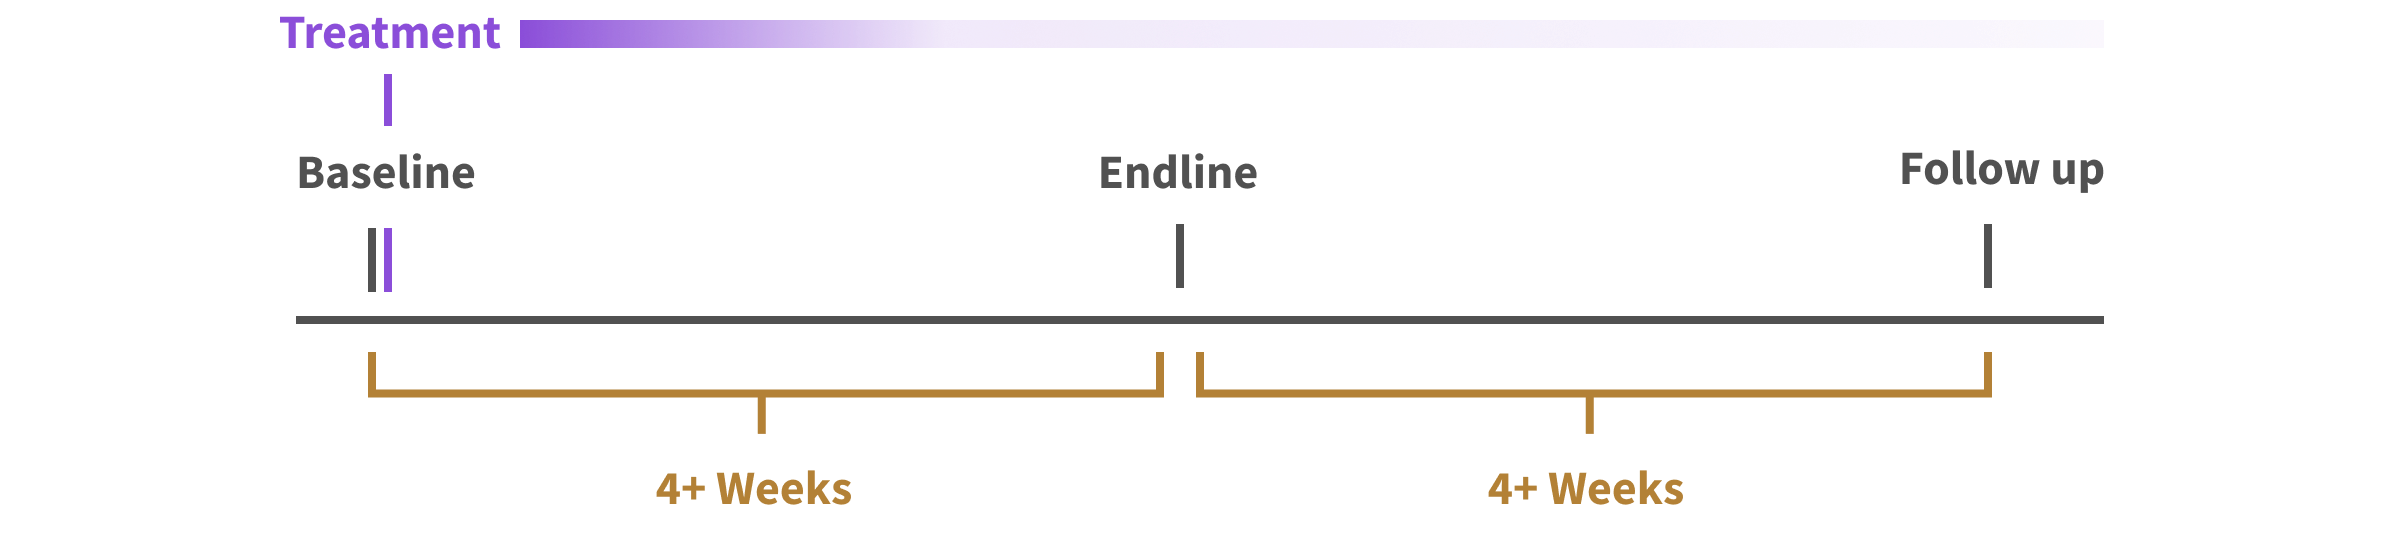
\includegraphics[width=\textwidth]{../images/design-timeline.png}
\caption{Study Design}
\label{fig:Study Design}
\end{figure}

\end{frame}

\section{Descriptives} 

\begin{frame}[shrink=10]
  \frametitle{Baseline Results}

  
% Table created by stargazer v.5.2.3 by Marek Hlavac, Social Policy Institute. E-mail: marek.hlavac at gmail.com
% Date and time: Sat, Feb 10, 2024 - 03:00:33 PM
% Requires LaTeX packages: dcolumn 
\begin{table}[!htbp] \centering 
  \caption{Outcome Construct Descriptives Pooled Baseline} 
  \label{tbl:Outcome Construct Descriptives Pooled Baseline} 
\begin{tabular}{@{\extracolsep{5pt}} D{.}{.}{-2} D{.}{.}{-2} D{.}{.}{-2} D{.}{.}{-2} D{.}{.}{-2} D{.}{.}{-2} D{.}{.}{-2} D{.}{.}{-2} } 
\\[-1.8ex]\hline 
\hline \\[-1.8ex] 
\multicolumn{1}{c}{name} & \multicolumn{1}{c}{mean} & \multicolumn{1}{c}{median} & \multicolumn{1}{c}{min} & \multicolumn{1}{c}{max} & \multicolumn{1}{c}{sd} & \multicolumn{1}{c}{prop\_max} & \multicolumn{1}{c}{prop\_na} \\ 
\hline \\[-1.8ex] 
\multicolumn{1}{c}{Activities Past 24h} & \multicolumn{1}{c}{4.92} & \multicolumn{1}{c}{5.0} & \multicolumn{1}{c}{0} & \multicolumn{1}{c}{6} & \multicolumn{1}{c}{1.23} & \multicolumn{1}{c}{0.41} & \multicolumn{1}{c}{0.00} \\ 
\multicolumn{1}{c}{Parenting Confidence} & \multicolumn{1}{c}{3.34} & \multicolumn{1}{c}{3.5} & \multicolumn{1}{c}{1} & \multicolumn{1}{c}{4} & \multicolumn{1}{c}{0.65} & \multicolumn{1}{c}{0.37} & \multicolumn{1}{c}{0.00} \\ 
\multicolumn{1}{c}{Positive Practices} & \multicolumn{1}{c}{3.20} & \multicolumn{1}{c}{3.5} & \multicolumn{1}{c}{1} & \multicolumn{1}{c}{4} & \multicolumn{1}{c}{0.75} & \multicolumn{1}{c}{0.27} & \multicolumn{1}{c}{0.00} \\ 
\multicolumn{1}{c}{Attitude to Phys. Punishment} & \multicolumn{1}{c}{3.13} & \multicolumn{1}{c}{3.0} & \multicolumn{1}{c}{1} & \multicolumn{1}{c}{4} & \multicolumn{1}{c}{0.84} & \multicolumn{1}{c}{0.36} & \multicolumn{1}{c}{0.00} \\ 
\multicolumn{1}{c}{Hostile Practices} & \multicolumn{1}{c}{3.04} & \multicolumn{1}{c}{3.0} & \multicolumn{1}{c}{1} & \multicolumn{1}{c}{4} & \multicolumn{1}{c}{0.69} & \multicolumn{1}{c}{0.15} & \multicolumn{1}{c}{0.00} \\ 
\multicolumn{1}{c}{Child Dev. Knowledge} & \multicolumn{1}{c}{0.86} & \multicolumn{1}{c}{1.0} & \multicolumn{1}{c}{0} & \multicolumn{1}{c}{1} & \multicolumn{1}{c}{0.28} & \multicolumn{1}{c}{0.73} & \multicolumn{1}{c}{0.00} \\ 
\multicolumn{1}{c}{Vaccine Knowledge} & \multicolumn{1}{c}{0.72} & \multicolumn{1}{c}{1.0} & \multicolumn{1}{c}{0} & \multicolumn{1}{c}{1} & \multicolumn{1}{c}{0.45} & \multicolumn{1}{c}{0.72} & \multicolumn{1}{c}{0.58} \\ 
\multicolumn{1}{c}{Breastfed} & \multicolumn{1}{c}{0.37} & \multicolumn{1}{c}{0.0} & \multicolumn{1}{c}{0} & \multicolumn{1}{c}{1} & \multicolumn{1}{c}{0.48} & \multicolumn{1}{c}{0.37} & \multicolumn{1}{c}{0.58} \\ 
\hline \\[-1.8ex] 
\end{tabular} 
\end{table} 


\end{frame}


\begin{frame}
    \frametitle{Baseline Results}

  Many of the constructs have quite high means and medians and some have a high proportion of respondents with the max score. In particular, 74\% and 75\% of respondents scored perfectly on the knowledge questions. 

This is problematic, as knowledge is often considered the easiest to change quickly and was a core outcome of interest for the team. Additionally, knowledge questions seem to be heavily impacted by the repeated survey effect, as discussed further down. 
\end{frame}



\begin{frame}[shrink=10]
 \frametitle{Attrition}


% Table created by stargazer v.5.2.3 by Marek Hlavac, Social Policy Institute. E-mail: marek.hlavac at gmail.com
% Date and time: Mon, Mar 11, 2024 - 09:43:37 PM
\begin{table}[H] \centering 
  \caption{Attrition: Pooled} 
  \label{tbl:Attrition: Pooled} 
\begin{tabular}{@{\extracolsep{5pt}} cccccc} 
\\[-1.8ex]\hline 
\hline \\[-1.8ex] 
stage & count & attrition & treated\_attrition & control\_attrition & attrition\_dif \\ 
\hline \\[-1.8ex] 
Started Baseline & 8994 &  &  &  &  \\ 
Finished Baseline & 4321 & 0.52 & 0.52 & 0.52 & 0.00 \\ 
Started Endline & 1968 & 0.54 & 0.54 & 0.55 & 0.00 \\ 
Finished Endline & 1679 & 0.15 & 0.17 & 0.13 & 0.04 \\ 
Started Followup &  569 & 0.66 & 0.66 & 0.66 & 0.00 \\ 
Finished Followup &  412 & 0.28 & 0.29 & 0.26 & 0.03 \\ 
\hline \\[-1.8ex] 
\end{tabular} 
\end{table} 


Given the high attrition and slow recruitment, the decision was made to focus on a pooled analysis of both countries. The treatment group experienced slightly higher attrition during surveys, possibly due to being asked more questions. However, the magnitude is relatively small.
\end{frame}

\begin{frame}
  \frametitle{Takeup}


\begin{figure}[H]
  \centering
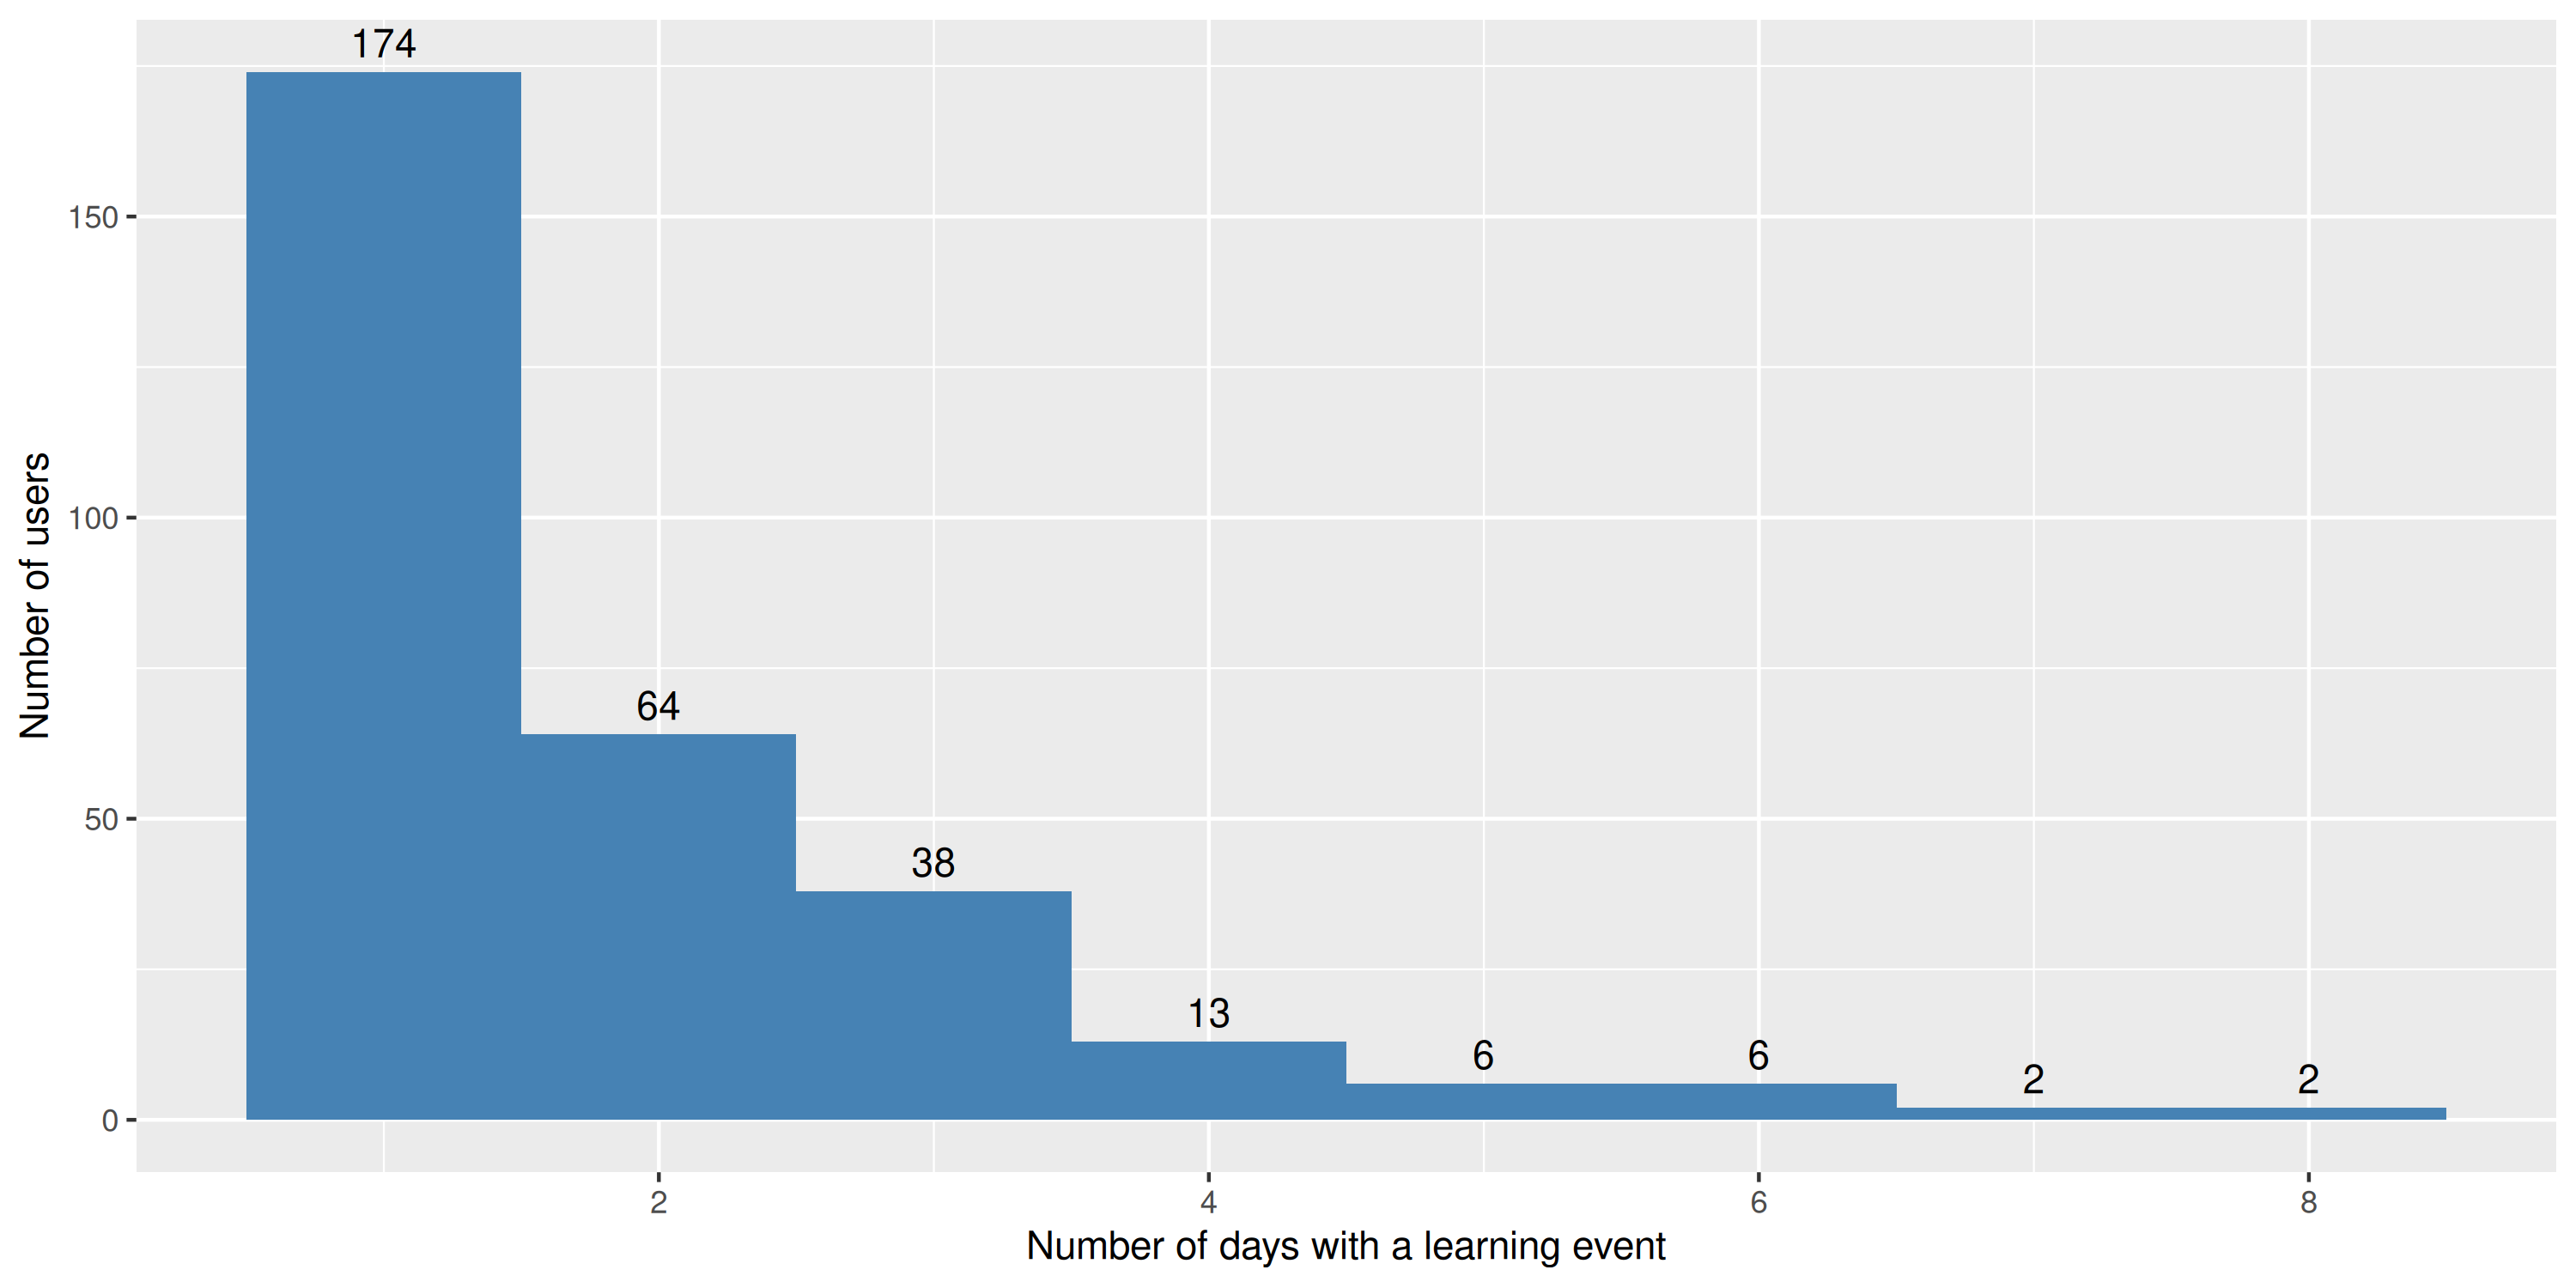
\includegraphics[width=0.9\textwidth]{../plots/Treatment Takeup Baseline - Endline.png}
\caption{Days with Learning Event (Baseline - Endline)}
\label{fig:treatment-takeup-histogram}
\end{figure}

\end{frame}

\begin{frame}[shrink=25]
  \frametitle{Takeup}


% Table created by stargazer v.5.2.3 by Marek Hlavac, Social Policy Institute. E-mail: marek.hlavac at gmail.com
% Date and time: Wed, Mar 20, 2024 - 10:37:13 PM
\begin{table}[H] \centering 
  \caption{Treatment Takeup} 
  \label{tbl:Treatment Takeup} 
\begin{tabular}{@{\extracolsep{5pt}} ccccccccc} 
\\[-1.8ex]\hline 
\hline \\[-1.8ex] 
Dataset & Treated & Downloaded & Used & \textgreater  1 Day & \textgreater  3 Days & Used (\%) & \textgreater  1 Day (\%) & \textgreater  3 Days (\%) \\ 
\hline \\[-1.8ex] 
Serbia &  678 & 379 & 189 &  85 & 18 & 27.9\% & 12.5\% & 2.7\% \\ 
Bulgaria &  342 & 182 & 116 &  46 & 11 & 33.9\% & 13.5\% & 3.2\% \\ 
Pooled & 1020 & 561 & 305 & 131 & 29 & 29.9\% & 12.8\% & 2.8\% \\ 
\hline \\[-1.8ex] 
\end{tabular} 
\end{table} 


The theory of change for Bebbo requires that individuals both download the app and use the app regularly. The evaluation assumption for this study was that by asking respondents to download Bebbo, a significant portion would download and regularly use the app. 

29.9\% downloaded and used the app once. This takeup is ``significant'' in the sense that we are powered in our study to measure an effect on this group. Unfortunately, most of those users never open the app beyond the first day. Only ~9\% of them open the app more than 3 days in the 4 weeks. 

\end{frame}


\begin{frame}[shrink=25]
  \frametitle{Takeup: External Validity}


% Table created by stargazer v.5.2.3 by Marek Hlavac, Social Policy Institute. E-mail: marek.hlavac at gmail.com
% Date and time: Mon, Mar 11, 2024 - 10:23:26 PM
\begin{table}[H] \centering 
  \caption{App Engagement (30 days)} 
  \label{tbl:App Engagement (30 days)} 
\begin{tabular}{@{\extracolsep{5pt}} ccccc} 
\\[-1.8ex]\hline 
\hline \\[-1.8ex] 
Dataset & Downloaded & Used (\%) & \textgreater  1 Day (\%) & \textgreater  3 Days (\%) \\ 
\hline \\[-1.8ex] 
Serbia &   340 & 50.3\% & 22.6\% & 4.4\% \\ 
Bulgaria &   162 & 64.2\% & 25.3\% & 6.2\% \\ 
Pooled &   497 & 54.7\% & 23.7\% & 5\% \\ 
Non-Study & 40111 & 26.7\% & 13.6\% & 5.1\% \\ 
\hline \\[-1.8ex] 
\end{tabular} 
\end{table} 


We can compare the app usage of our participants to the app usage data from non-study participants to assess whether or not this is representative of real-world app usage. While we find that our study participants are more likely to finish onboarding (use) and more likely to use beyond the first day, they are equally likely to become regular users.

\end{frame}



\begin{frame}
  \frametitle{Power}

Ex-post power analysis shows that we are well powered (above 80\% power at a 1.25\% significance level) with around 2000 participants in the pooled sample to find a medium effect size (0.5 standard deviations) at endline on those who downloaded and used Bebbo at least once (29.9\% takeup).

While it might be of interest to examing the treatment effect on the small subset of regular users, doing so in a randomized control trial, with this power, would require 227,576 study participants (at 2.8\% takeup). Even to measure the impact on those who used it at least two days would require 10,892 participants to be equally powered. 

\end{frame}

\begin{frame}
  \frametitle{Bottom line}

Asking participants to download and use Bebbo did not cause a significant portion of them to use it regularly.

Thus, we will be able to evaluate the impact of downloading and using Bebbo once, but not the impact of ``regular'' Bebbo usage.

\end{frame}

\section{Findings}

\begin{frame}
\frametitle{Findings}
 
The analysis conducted on the effects of promoting the Bebbo app on caregivers with children aged 0-6 did not reveal any statistically significant impact on key outcomes of interest. 

\end{frame}


\begin{frame}
   \frametitle{Findings}
One of the main contributing factors that aligns with the theory of change is the low engagement levels of users with the app: without regular usage, we would expect no impact. Additional findings that might have contributed to the lack of measured significant impact include: 

  \begin{enumerate}
  \item There seemed to be a priming effect of the baseline survey, especially for questions related to knowledge, such as “when is your child’s next vaccination due.” This could imply that a prompt itself can change parent’s knowledge and raises questions on how best to position Bebbo in regards to this outcome. 
  \item The majority of respondents scored well on the baseline assessment. If the respondents were representative of the general population, this would imply that most caregivers in these countries are already knowledgeable and following many good practices.
  \end{enumerate}
    
\end{frame}

\begin{frame}
 \frametitle{Findings: App Usage}

Given that so few caregivers used the app, it seems important to ask the question: “who are the respondents who end up as app users?” We do so by regressing respondents’ app usage activity against their characteristics at baseline. 

Unfortunately, we are not able to accurately predict engagement from the measured baseline characteristics.

One notable predictor is ``Activities Past 24h.'' One possible interpretation could be that there is a set of people who are not likely to spend time with their children but are likely to download and use apps. Unfortunately, the raw data is not reflective of a positive impact of this app on those people spending more time with their children. There is some additional evidence that those with young children are more likely to become regular users of the app as well as those who are parents (compared to other caregivers). 
\end{frame}

\section{Suggestive Evidence}

\begin{frame}
  \frametitle{Suggestive Evidence}

We are not able to detect a significant impact of treatment in this randomized control trial. However, it can be useful to examine the raw before-and-after data for suggestive evidence to be explored further in future research. 

Note that before-and-after data does not represent the impact of usage, as users ``self-select'' into the group who uses the app. In other words: those who use the app more than 3 times do so for some reason, potentially because they are eager to learn or change. This group may have learned or changed with or without the app. Thus, what we are uncovering is correlation, not causation. 

\end{frame}

\begin{frame}
 \frametitle{Suggestive Evidence: Knowledge and Awareness}
There is evidence that awareness itself drives vaccine knowledge improvement. There is some suggestive evidence that regular app usage is correlated with increased knowledge and confidence in knowledge about child development stages. 
\begin{figure}[H]
  \centering
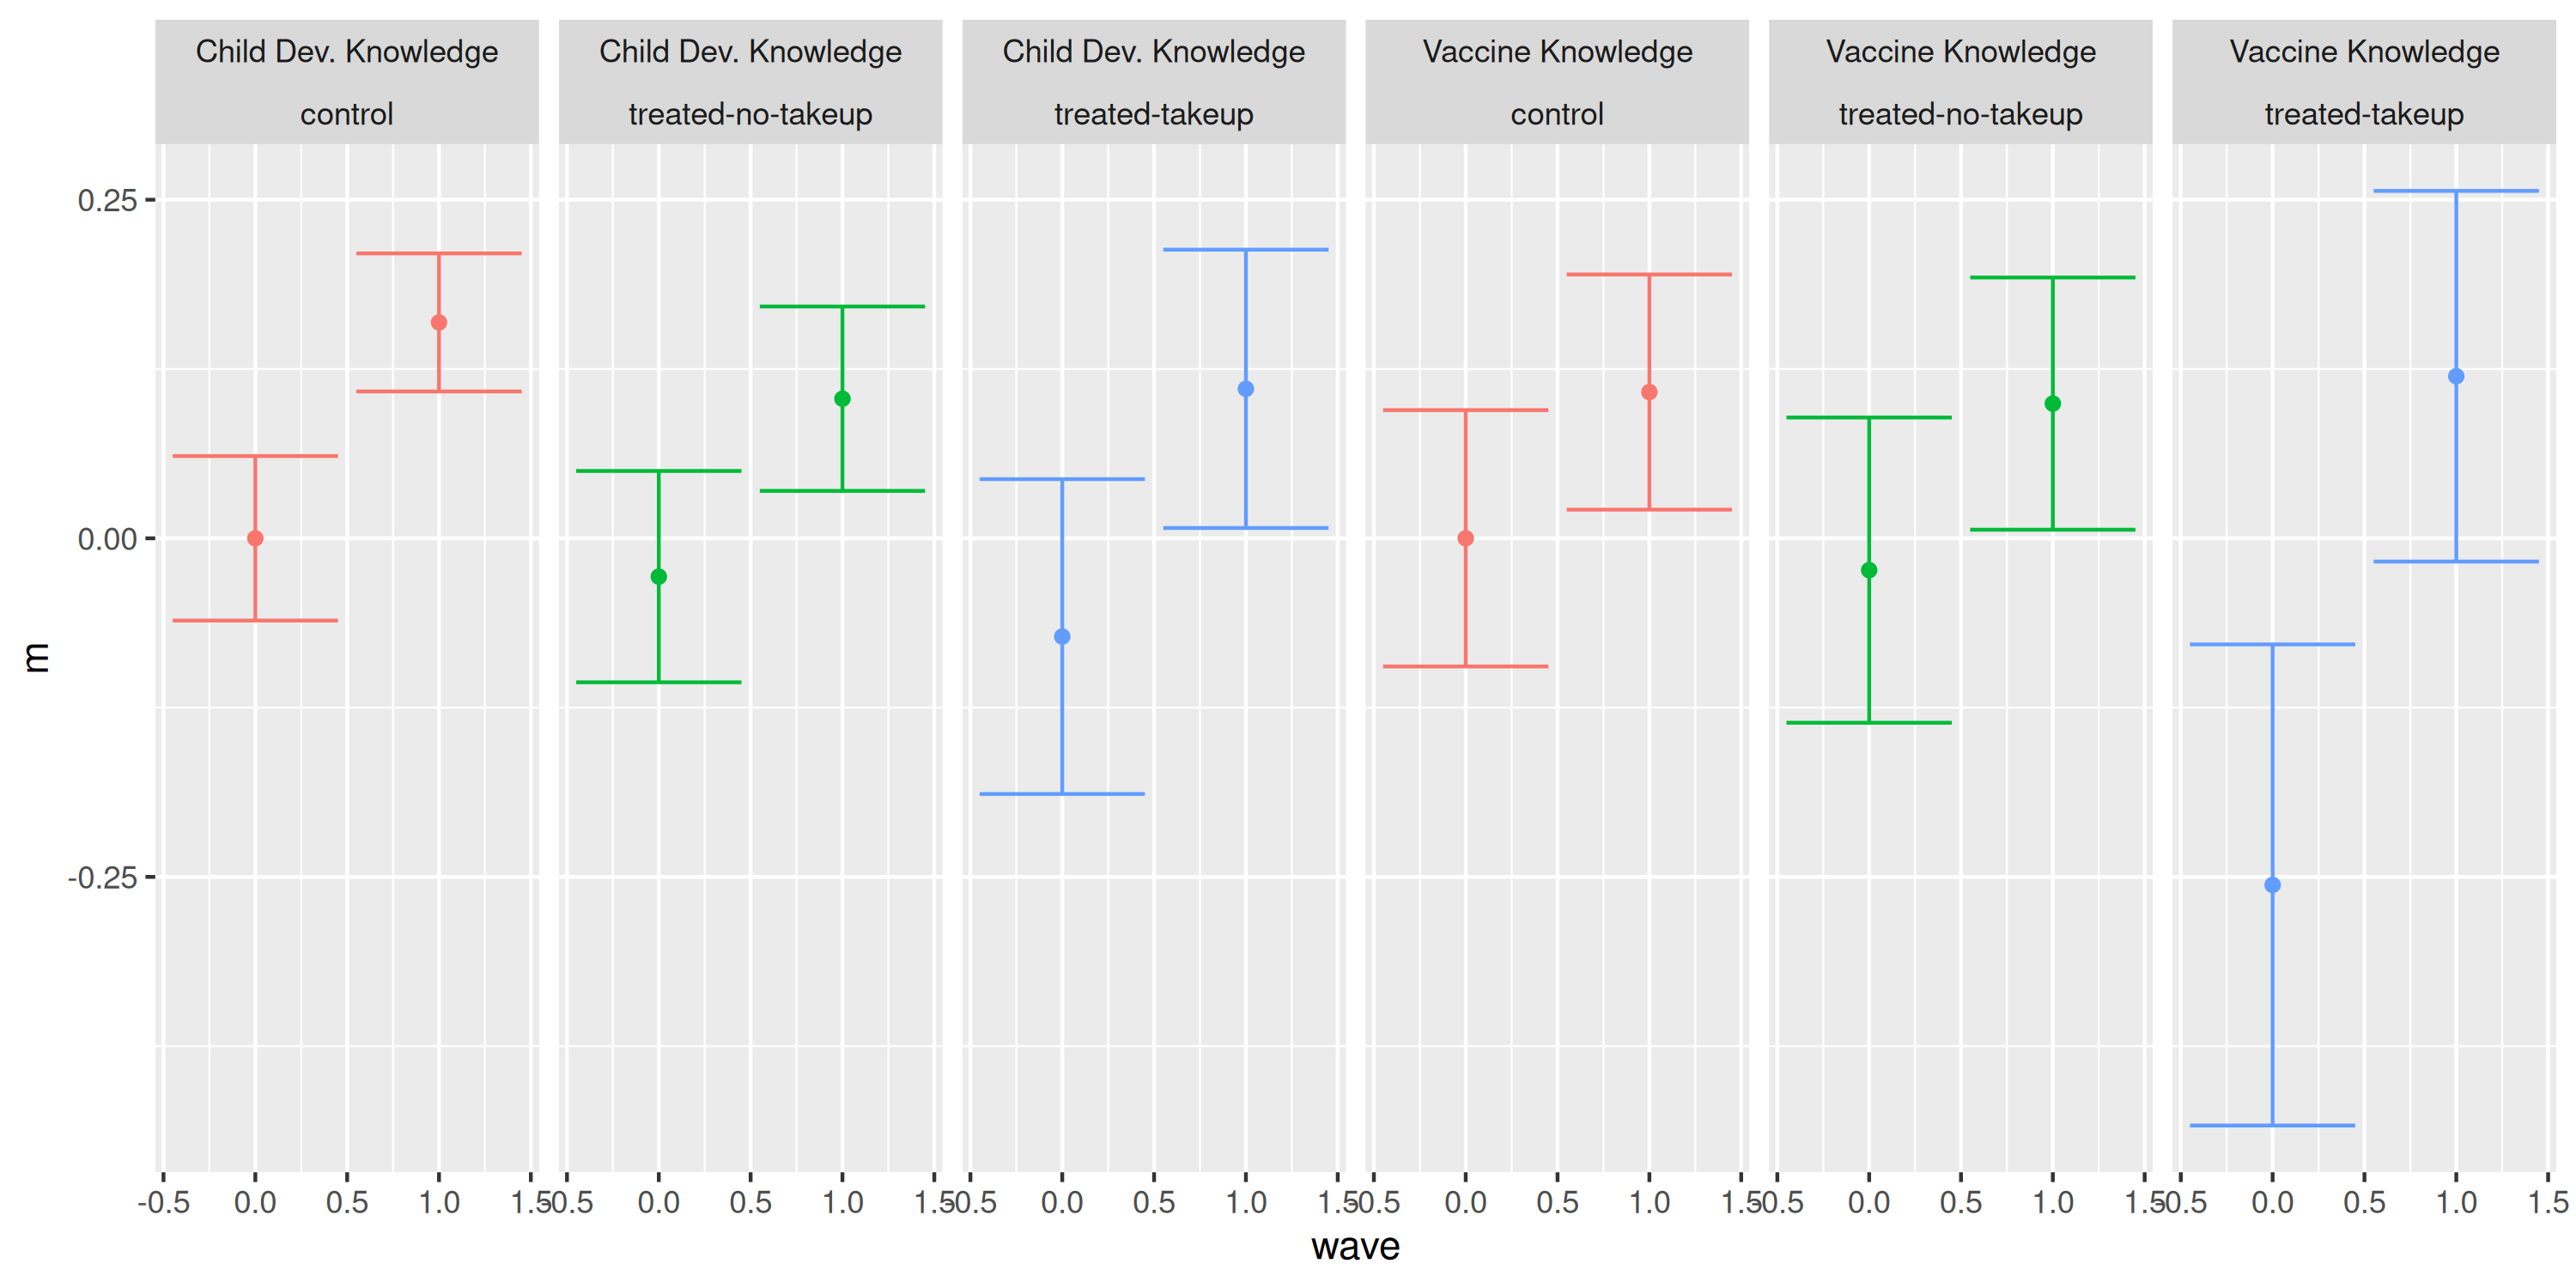
\includegraphics[width=\textwidth]{../plots/pre_post/Pooled: Vaccine Knowledge.png}
\label{fig:knowledge-pre-post}
\end{figure}
   
\end{frame}

\begin{frame}
 \frametitle{Suggestive Evidence: Confidence and Attitudes}

There is evidence that regular app usage is correlated with improved confidence and attitudes towards physical punishment. 
\begin{figure}[H]
  \centering
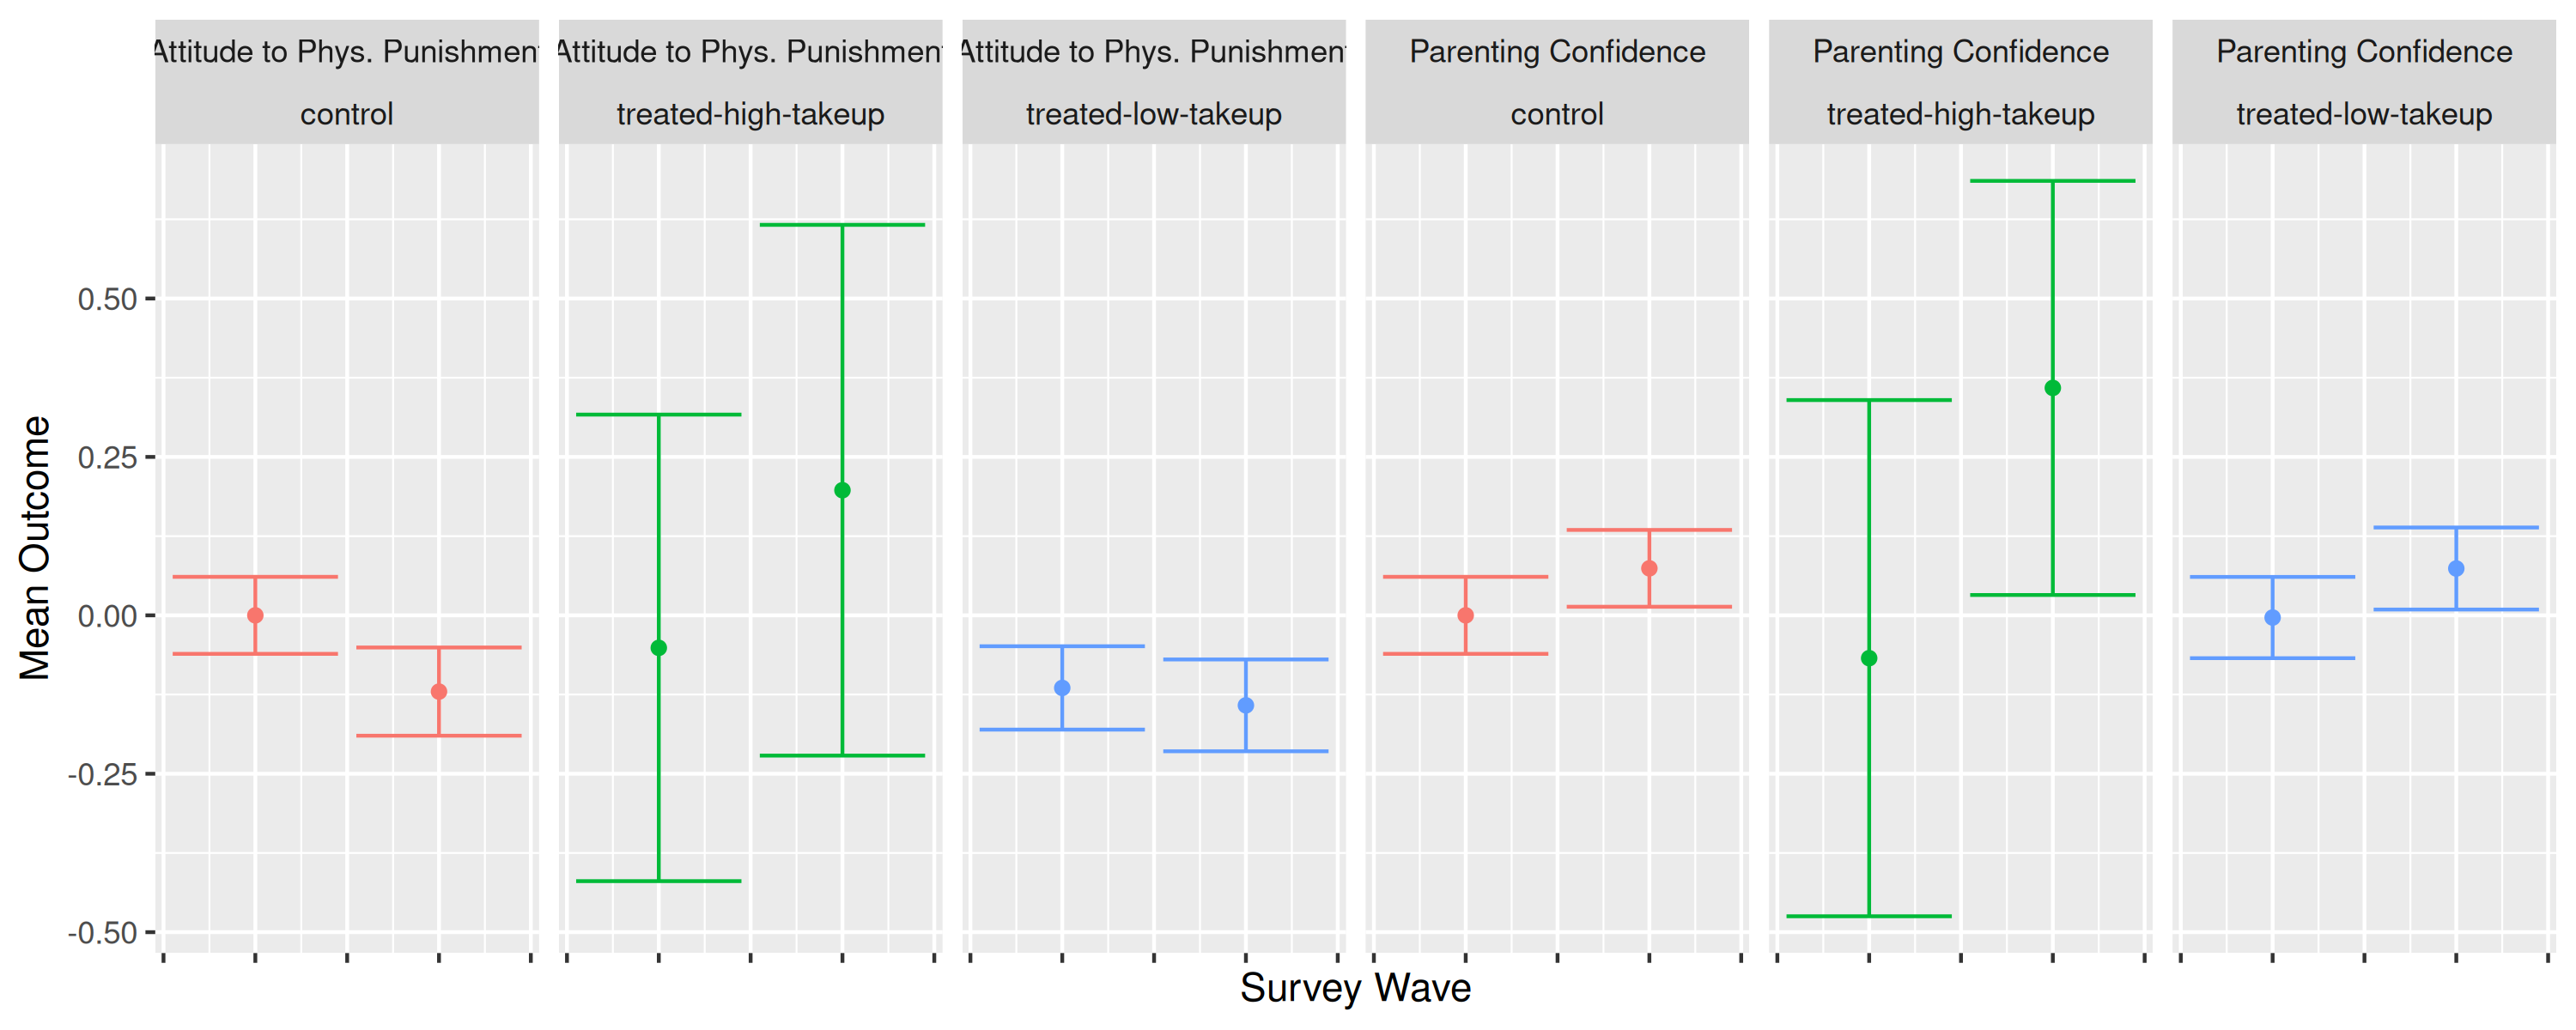
\includegraphics[width=\textwidth]{../plots/pre_post/Pooled: Parenting Confidence.png}
\label{fig:confidence-and-attitudes-pre-post}
\end{figure}
   
\end{frame}


\begin{frame}
 \frametitle{Suggestive Evidence: Practices}
There is evidence that regular app usage is correlated with spending less time with their child in important activities and seems independent of breastfeeding. 

\begin{figure}[H]
  \centering
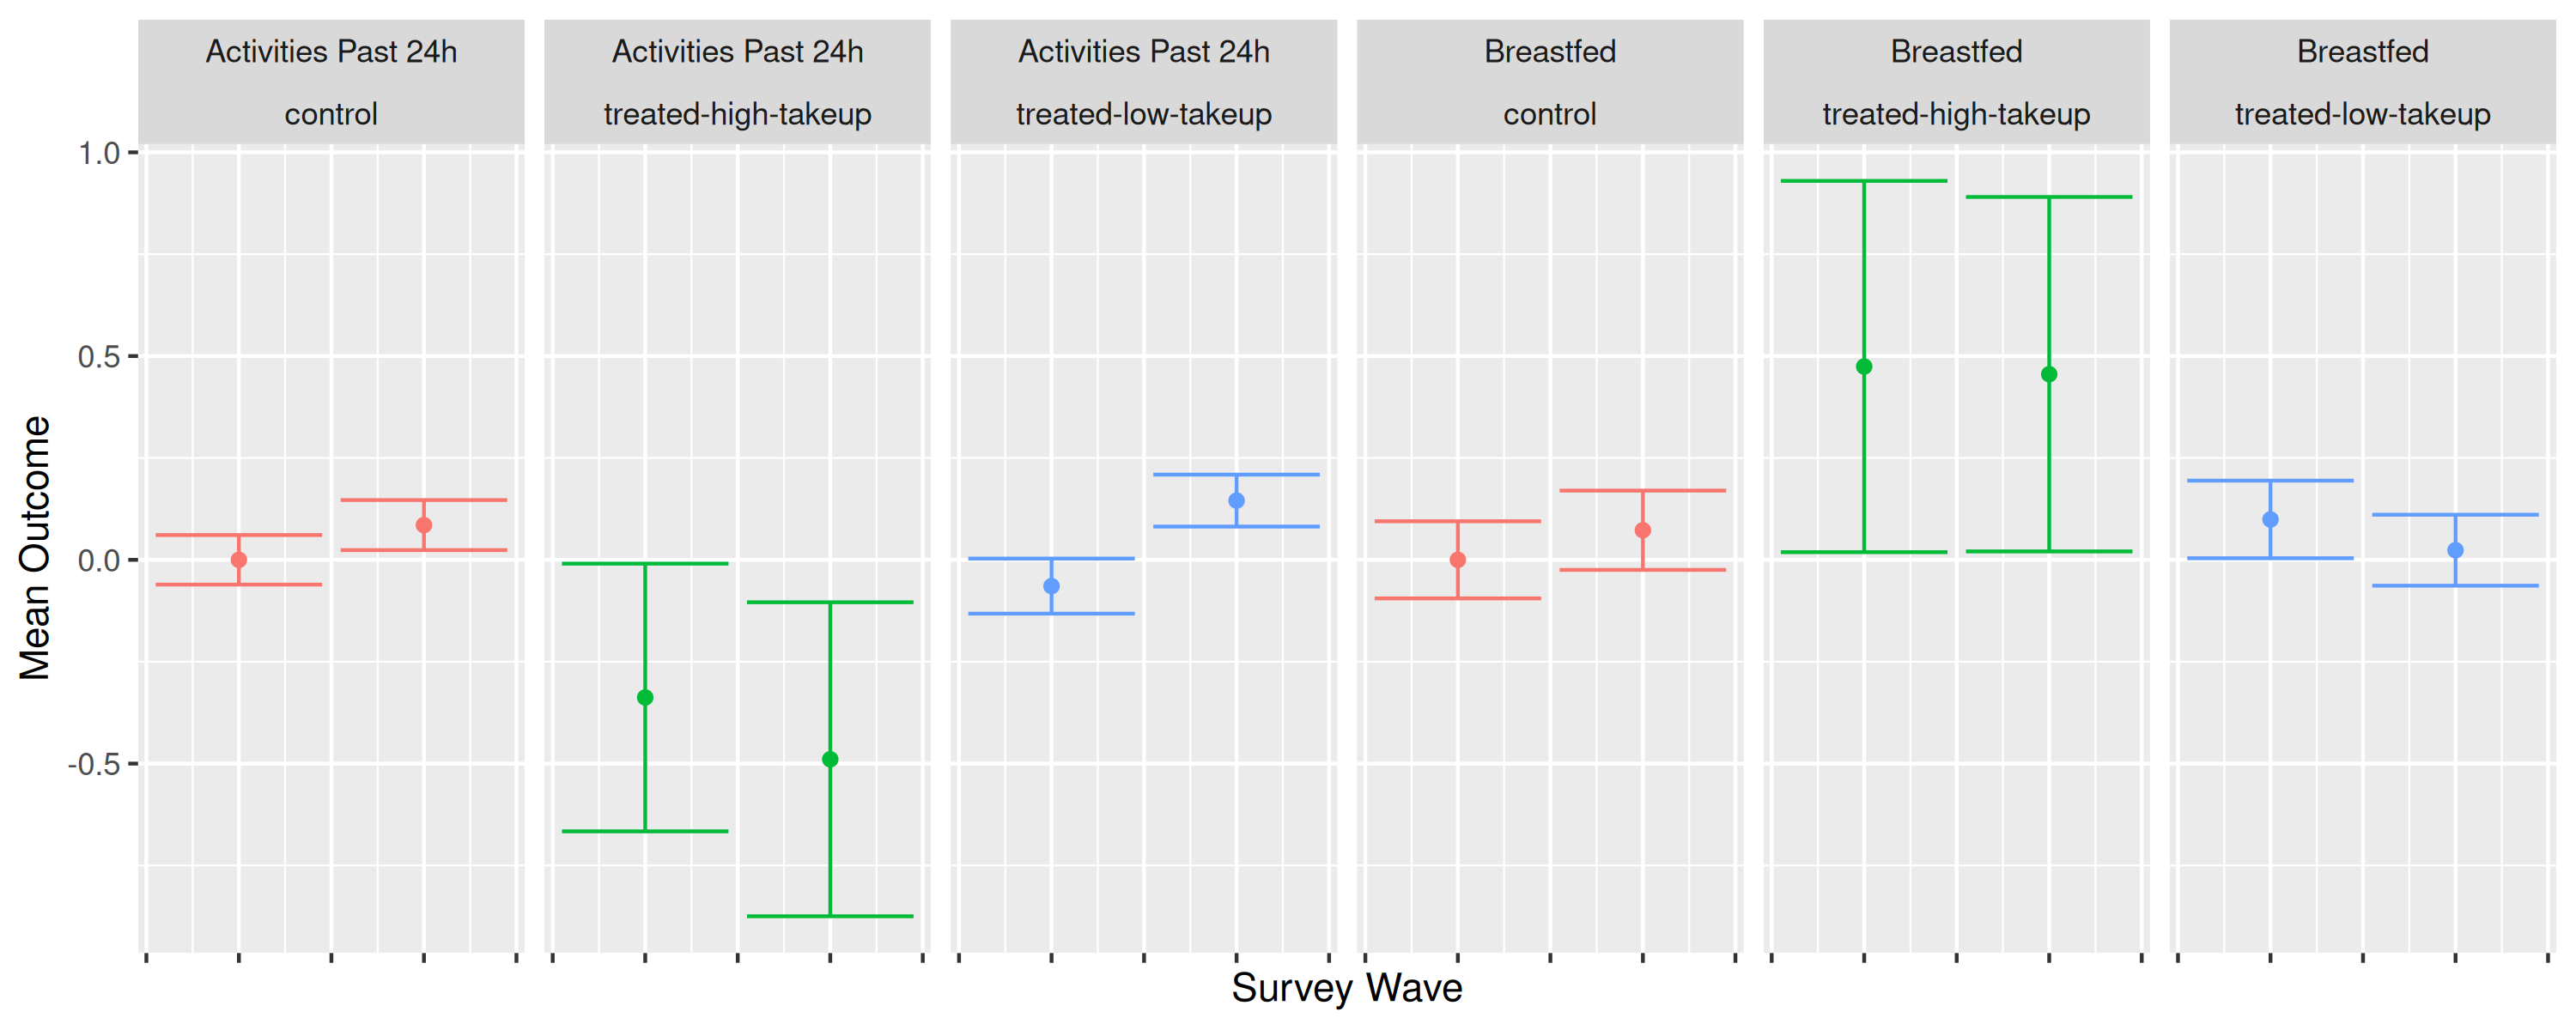
\includegraphics[width=0.9\textwidth]{../plots/pre_post/Pooled: Breastfed.png}
\label{fig:practices-pre-post}
\end{figure}
   
\end{frame}


\begin{frame}
 \frametitle{Suggestive Evidence: Practices}

There is evidence that regular app usage is correlated with improved positive parenting practices. 
\begin{figure}[H]
  \centering
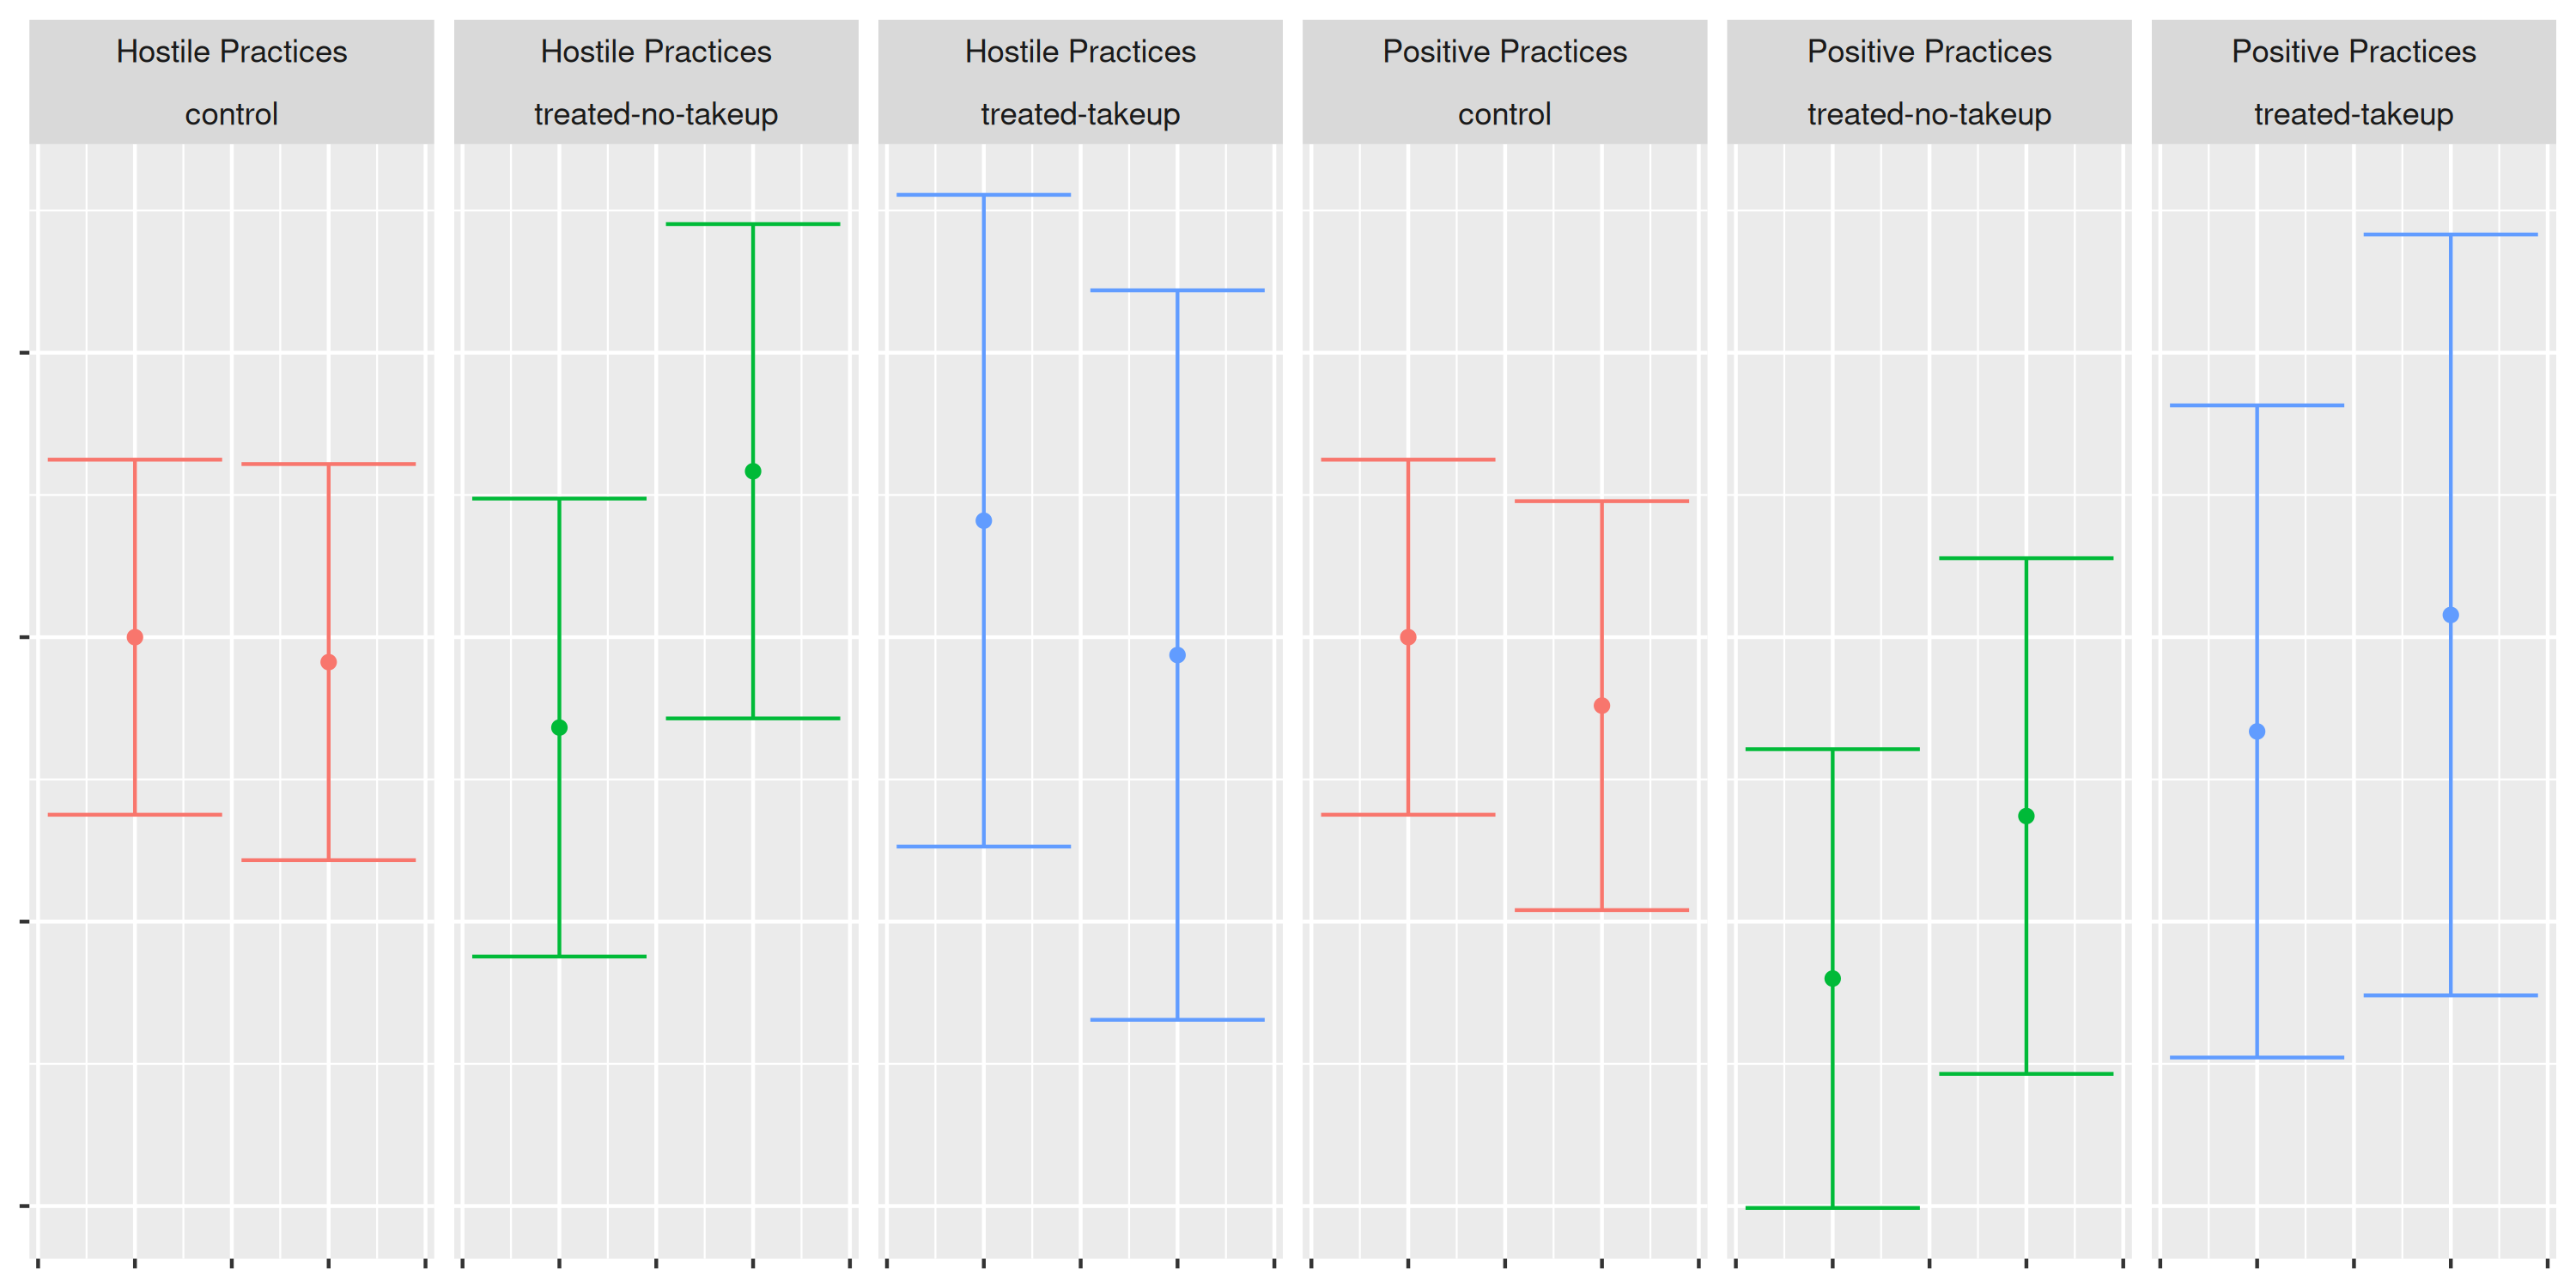
\includegraphics[width=0.9\textwidth]{../plots/pre_post/Pooled: Positive Practices.png}
\label{fig:practices-pre-post}
\end{figure}
   
\end{frame}


\section{Recommendations}


\begin{frame}
   \frametitle{Recommendations}

For an app to influence behaviors and attitudes, it must be attractive and engaging enough to retain a large portion of the target audience over time. 

Data indicate that a significant proportion of users tend to abandon the app after a short period. Specifically, 76\% of users in our study who complied with the suggestion to download Bebbo abandoned it after the first day. This is in line with app usage data outside of our study, which shows that over 80\% of users abandon it after one day. 

We additionally find that only 3\% of respondents used Bebbo more than 3 times in a 30 day period. Bebbo’s theory of change is anchored in regular app usage by parents – the current usage rate is unlikely to lead to impact change.

\end{frame}

\begin{frame}
   \frametitle{Recommendations}

\textbf{Improve app targeting}

The 5\% of downloaders that remain as regular users, as well as other suggestive evidence, indicate that Bebbo may work for specific sub-groups. These groups need to be better understood to improve app outreach and uptake strategies. Unfortunately, we were not able to learn much about this subgroup in this analysis. It might be that new implementation modalities would be required to reach these groups. The current shift towards implementing through services providers (i.e., a hybrid strategy) might provide a solution, but it needs to be tested before being scaled up.  

\end{frame}

\begin{frame}
   \frametitle{Recommendations}

\textbf{Adjust app focus based on context}

Considering the high baseline scores of participants, it might be valuable (in places with already better than average parenting knowledge) to consider a focus on particular practices (i.e. breastfeeding) that are still lagging, or groups which are lagging in all practices. 
\end{frame}

\begin{frame}
   \frametitle{Recommendations}
 

\textbf{Adjust app focus based on the comparative advantage to generate knowledge}

The findings suggest that  for many of the targeted outcomes, awareness itself is an effective intervention. This suggests that some outcomes (such as vaccine knowledge) might be more effective through other media and an app should focus on the outcomes that require sustained engagement. 
\end{frame}

\begin{frame}
     \frametitle{Recommendations}
\textbf{Improve app usage}

The current retention and usage rates are not sufficient for Bebbo to have any meaningful impact. Steps should be taken to make the app more engaging for caregivers (and service providers considering the new implementation modality). These implementation issues should be addressed through formative and quantitative research  (e.g., User experience (UX) studies to understand what would drive better user engagement, acceptability, accessibility, and reach) before further scaling the app.  

\end{frame}

\begin{frame}
\frametitle{Recommendations}       

\textbf{Adopt a lean approach to product development}

Continuous user testing, lean UX techniques, and agile development methodologies should be used to define and test the core assumptions to the theory of change of an intervention. In this particular case, existing app usage data provided clear evidence of the biggest bottleneck: user onboarding and profile creation. Adopting continuous hypothesis testing from lean methodologies provides a framework to efficiently uncover these issues. 

\end{frame}


\begin{frame}
\frametitle{Recommendations}       

\textbf{Adopt a lean approach to evaluation}

Continuous evaluation can and should be woven in to every stage of the development lifecycle. Evaluation teams or tools can be used to assist the product team in testing hypotheses that are core to the theory of change of the intervention.

\end{frame}


\begin{frame}
   \frametitle{Findings and Recommendations}

  In conclusion, while the promotion of the Bebbo app did not result in significant effects on the target population, the study provides valuable insights into the challenges of promoting and sustaining engagement with mobile apps for parenting. 

Future interventions should consider strategies to enhance user engagement and retention to maximize the potential impact of mobile apps in promoting positive parenting practices and knowledge. 
\end{frame}

\end{document}

%------------------------------------------------